\documentclass[11pt,a4paper,twoside]{article}
\usepackage[utf8]{inputenc}
\usepackage[french]{babel}
\usepackage[T1]{fontenc}
\usepackage{graphicx}
\usepackage{charter}
\usepackage{hyperref}
\usepackage{listings}
\usepackage{wrapfig}
\usepackage[left=2cm,right=2cm,top=2cm,bottom=2cm]{geometry}
\setlength{\headheight}{15pt}
\usepackage{fancyhdr}
\pagestyle{fancy}
\usepackage{lastpage}
\renewcommand\headrulewidth{1pt}
\fancyhead[L]{Dossier Technique}
\renewcommand\footrulewidth{1pt}
\fancyfoot[C]{\textbf{Page \thepage/\pageref{LastPage}}}
\author{Mylann Dupuy}
\title{Dossier Technique --  \\ Powered by \LaTeX}
\date{30 Mars 2019 - Version 2.0}

\setlength{\parindent}{0cm}
\setlength{\parskip}{1ex plus 0.5ex minus 0.2ex}
\newcommand{\hsp}{\hspace{20pt}}
\newcommand{\HRule}{\rule{\linewidth}{0.5mm}}
\begin{document}

\begin{titlepage}
  \begin{sffamily}
  \begin{center}

    \textsc{\LARGE Dossier Technique - Powered by \LaTeX}\\[6.5cm]
    
\includegraphics[scale=1]{Ressources/polysoude.jpg}
    % Title
        \HRule \\[0.4cm]
        { \huge \bfseries TECHNICIEN SUPÉRIEUR DE SUPPORT INFORMATIQUE\\[0.4cm] }

        \HRule \\[6.5cm]

    % Author and supervisor
    \begin{minipage}{0.4\textwidth}
      \begin{flushleft} \large
        Candidat : Mylann \textsc{Dupuy}\\
        Promotion : HAPPT201\\
        Titre : T2SI
      \end{flushleft}
    \end{minipage}
    \begin{minipage}{0.5\textwidth}
      \begin{flushright} \large
        \emph{Tuteur :} M. Olivier \textsc{Naud}\\
        \emph{Binôme :} M. Antoine \textsc{Etrillard}\\
      \end{flushright}
    \end{minipage}

    \vfill

    % Bottom of the page
    {\large Version 2.0 - 05 Mars 2019}

  \end{center}
  \end{sffamily}
\end{titlepage}
\newpage

% ##### Page 3 #####
\tableofcontents
\newpage
%\setcounter{page}{3}
\newpage

% ##### Page 5 #####
\section{Introduction}
Avant de parler de moi, je souhaiterais remercier l'entreprise qui m'a accueilli, il s'agit de \textbf{POLYSOUDE} ainsi qu'à l'équipe informatique qui me supporte depuis \textbf{Septembre 2017} au sein de leur service.

\subsection{Mon parcours}
Venant d'un \textbf{BAC PRO SEN} (Systèmes Électroniques Numériques) d'un lycée professionnel au Mans (72), j'ai poursuivi un \textbf{BTS SIO} que j'ai abandonné pour finalement être au sein de l'\textbf{ENI} depuis septembre 2017 pour le titre \textbf{BAC +2 T2SI}

\subsection{Pourquoi cette formation et pas une autre ?}

C'est en recherchant une nouvelle formation que j'ai découvert l'existence du centre de formation de l'\textbf{ENI}.\\

En lisant les points qui allaient être étudier pendant la \textbf{formation T2SI} (qui m'était inconnue à ce jour), cela se rapprocher de ce que j'avais découvert pendant le BTS SIO mais sans les matières générales et qui m'a aussi permis d'en apprendre davantage. \\
\\
L'objectif que j'ai entrepris quand j'ai été accepté pour cette formation est de pouvoir décrocher le titre et ainsi intégrer une entreprise avec une possibilité d'évolution (dans le futur) avec un renouveau de mes connaissances et une ouverture d'esprit sur l'apprentissage et pour le travail en équipe.
\newpage

% ##### Page 4 #####
\section{Présentation de l'entreprise}
L'entreprise POLYSOUDE a été fondée en 1961 en se disant "pionnière dans la conception et la fabrication de matériel de soudage orbital". En 58 ans d'existence, l'entreprise a ouverte diverses filiales à travers le monde.\\

Aujourd'hui, la maison mère de POLYSOUDE basée à Nantes compte 300 employés à son actif ainsi que 12 filiales / bureaux sans oublier les partenaires à travers le monde (+ de 50 partenaires). \\

Toutes les informations concernant POLYSOUDE sont disponible ici : \textbf{\hyperlink{https://www.polysoude.com/}{Lien Internet}}

\subsection{Hiérarchie}
L'organigramme ci-dessous résume en grande partie tous les différents départements que l'on peut y trouver actuellement.
\begin{figure}[h!]
  \centering
  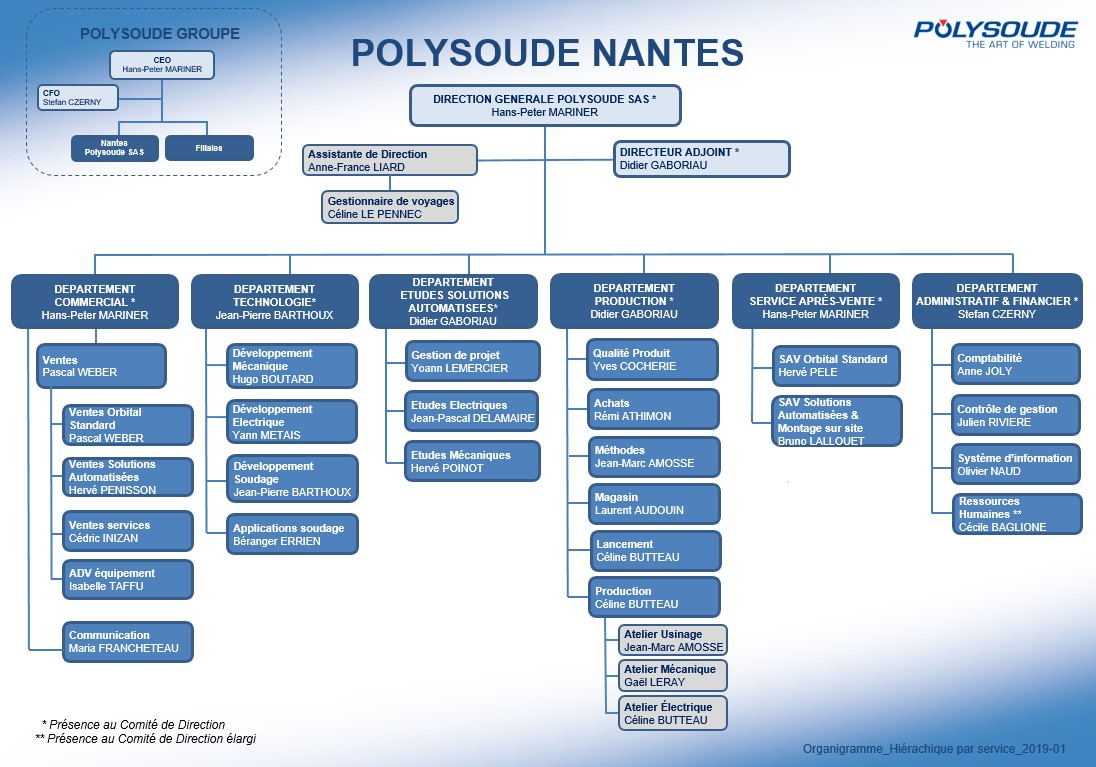
\includegraphics[width=\linewidth]{Ressources/Organigramme.jpg}
  \caption{Organigramme}
\end{figure}

Dans mon cas, mon collègue, \textbf{Antoine ETRILLARD} et moi-même somment dirigé par \textbf{Olivier NAUD} qui lui-même est dirigé par \textbf{Stefan CZERNY}.
\newpage

% ##### Page 5 #####
\section{Présentation de l'informatique dans l'entreprise}
\subsection{L'équipe}
Avant de parler de l'infrastructure, je vais nommer les membres qui composent l'ensemble du service IT car chaque collaborateur à un rôle à jouer que ce soit pour les logiciels métiers comme pour l'assistance aux utilisateurs.

\begin{itemize}
    \item \textbf{Olivier NAUD :} Le responsable du Service IT s'occupe principalement de l'administration système et réseau de l'entreprise (Gestion des droits O365, infra, Téléphonie, etc...) avec l'aide de diverses prestataires. \\
    %%%%%%%%%%
    \item \textbf{Vanessa PELLE :} Cette collaboratrice s'occupe de l'ERP \footnote{Enterprise Resource Planning} nommé \hyperlink{https://www.ifsworld.com/fr/}{IFS} en formant les utilisateurs, traite les incidents et les demandes liés à l'ERP. \\
    %%%%%%%%%%
    \item \textbf{Maxime CLAVIER :} Ce collaborateur s'occupe du logiciel métier, la solution \hyperlink{https://www.solidworks.com/fr}{SOLIDWORKS} \footnote{Logiciel de conception CAO 3D} ainsi que la solution de planning \hyperlink{https://www.visual-planning.com/fr/}{VISUAL PLANNING ou VP}. en faisant aussi des formations et de la résolution de problèmes lié à cette suite.\\
    %%%%%%%%%%
    \item \textbf{Antoine ETTRILLARD :} 1\ier{} pilier du service IT, il traite les demandes d'appels / mails en créant les tickets GLPI \footnote{Gestion Libre de Parc Informatique} puis assiste les utilisateurs pour la résolution de leur(s) problème(s) et/ou demande(s).
\end{itemize}
   
\subsection{Matériels}
L'infrastructure est gérée en interne, je m'explique :

\begin{itemize}
    \item \textbf{Serveurs :} Qu'ils soient physiques ou virtuels (sous un hyperviseur de type 1 : \textbf{Hyver-V)}, ils sont gérés par notre responsable et sous contrat chez différents prestataires / revendeurs. Tout les serveurs sont basés sur Windows Server (2008, 2012 R2).\\
    %%%%%%%%%%
    \item \textbf{Clients :} Les différents collaborateurs de l'entreprise utilisent tous une machine réelle que ce soit un poste fixe ou un poste portable. Une liste exhaustive est présente ci-dessous. Les clients utilisent Windows 7 ou Windows 10. \\
\end{itemize}
Dans l'ensemble des serveurs présents, ils sont dupliqués et/ou sauvegardés vers le site distant (Data Center) 
    
Dû à la limite de page imposée pour ce dossier, je ne parlerai donc que des postes clients.
\newpage

% Schéma réseau
\rotatebox{90}{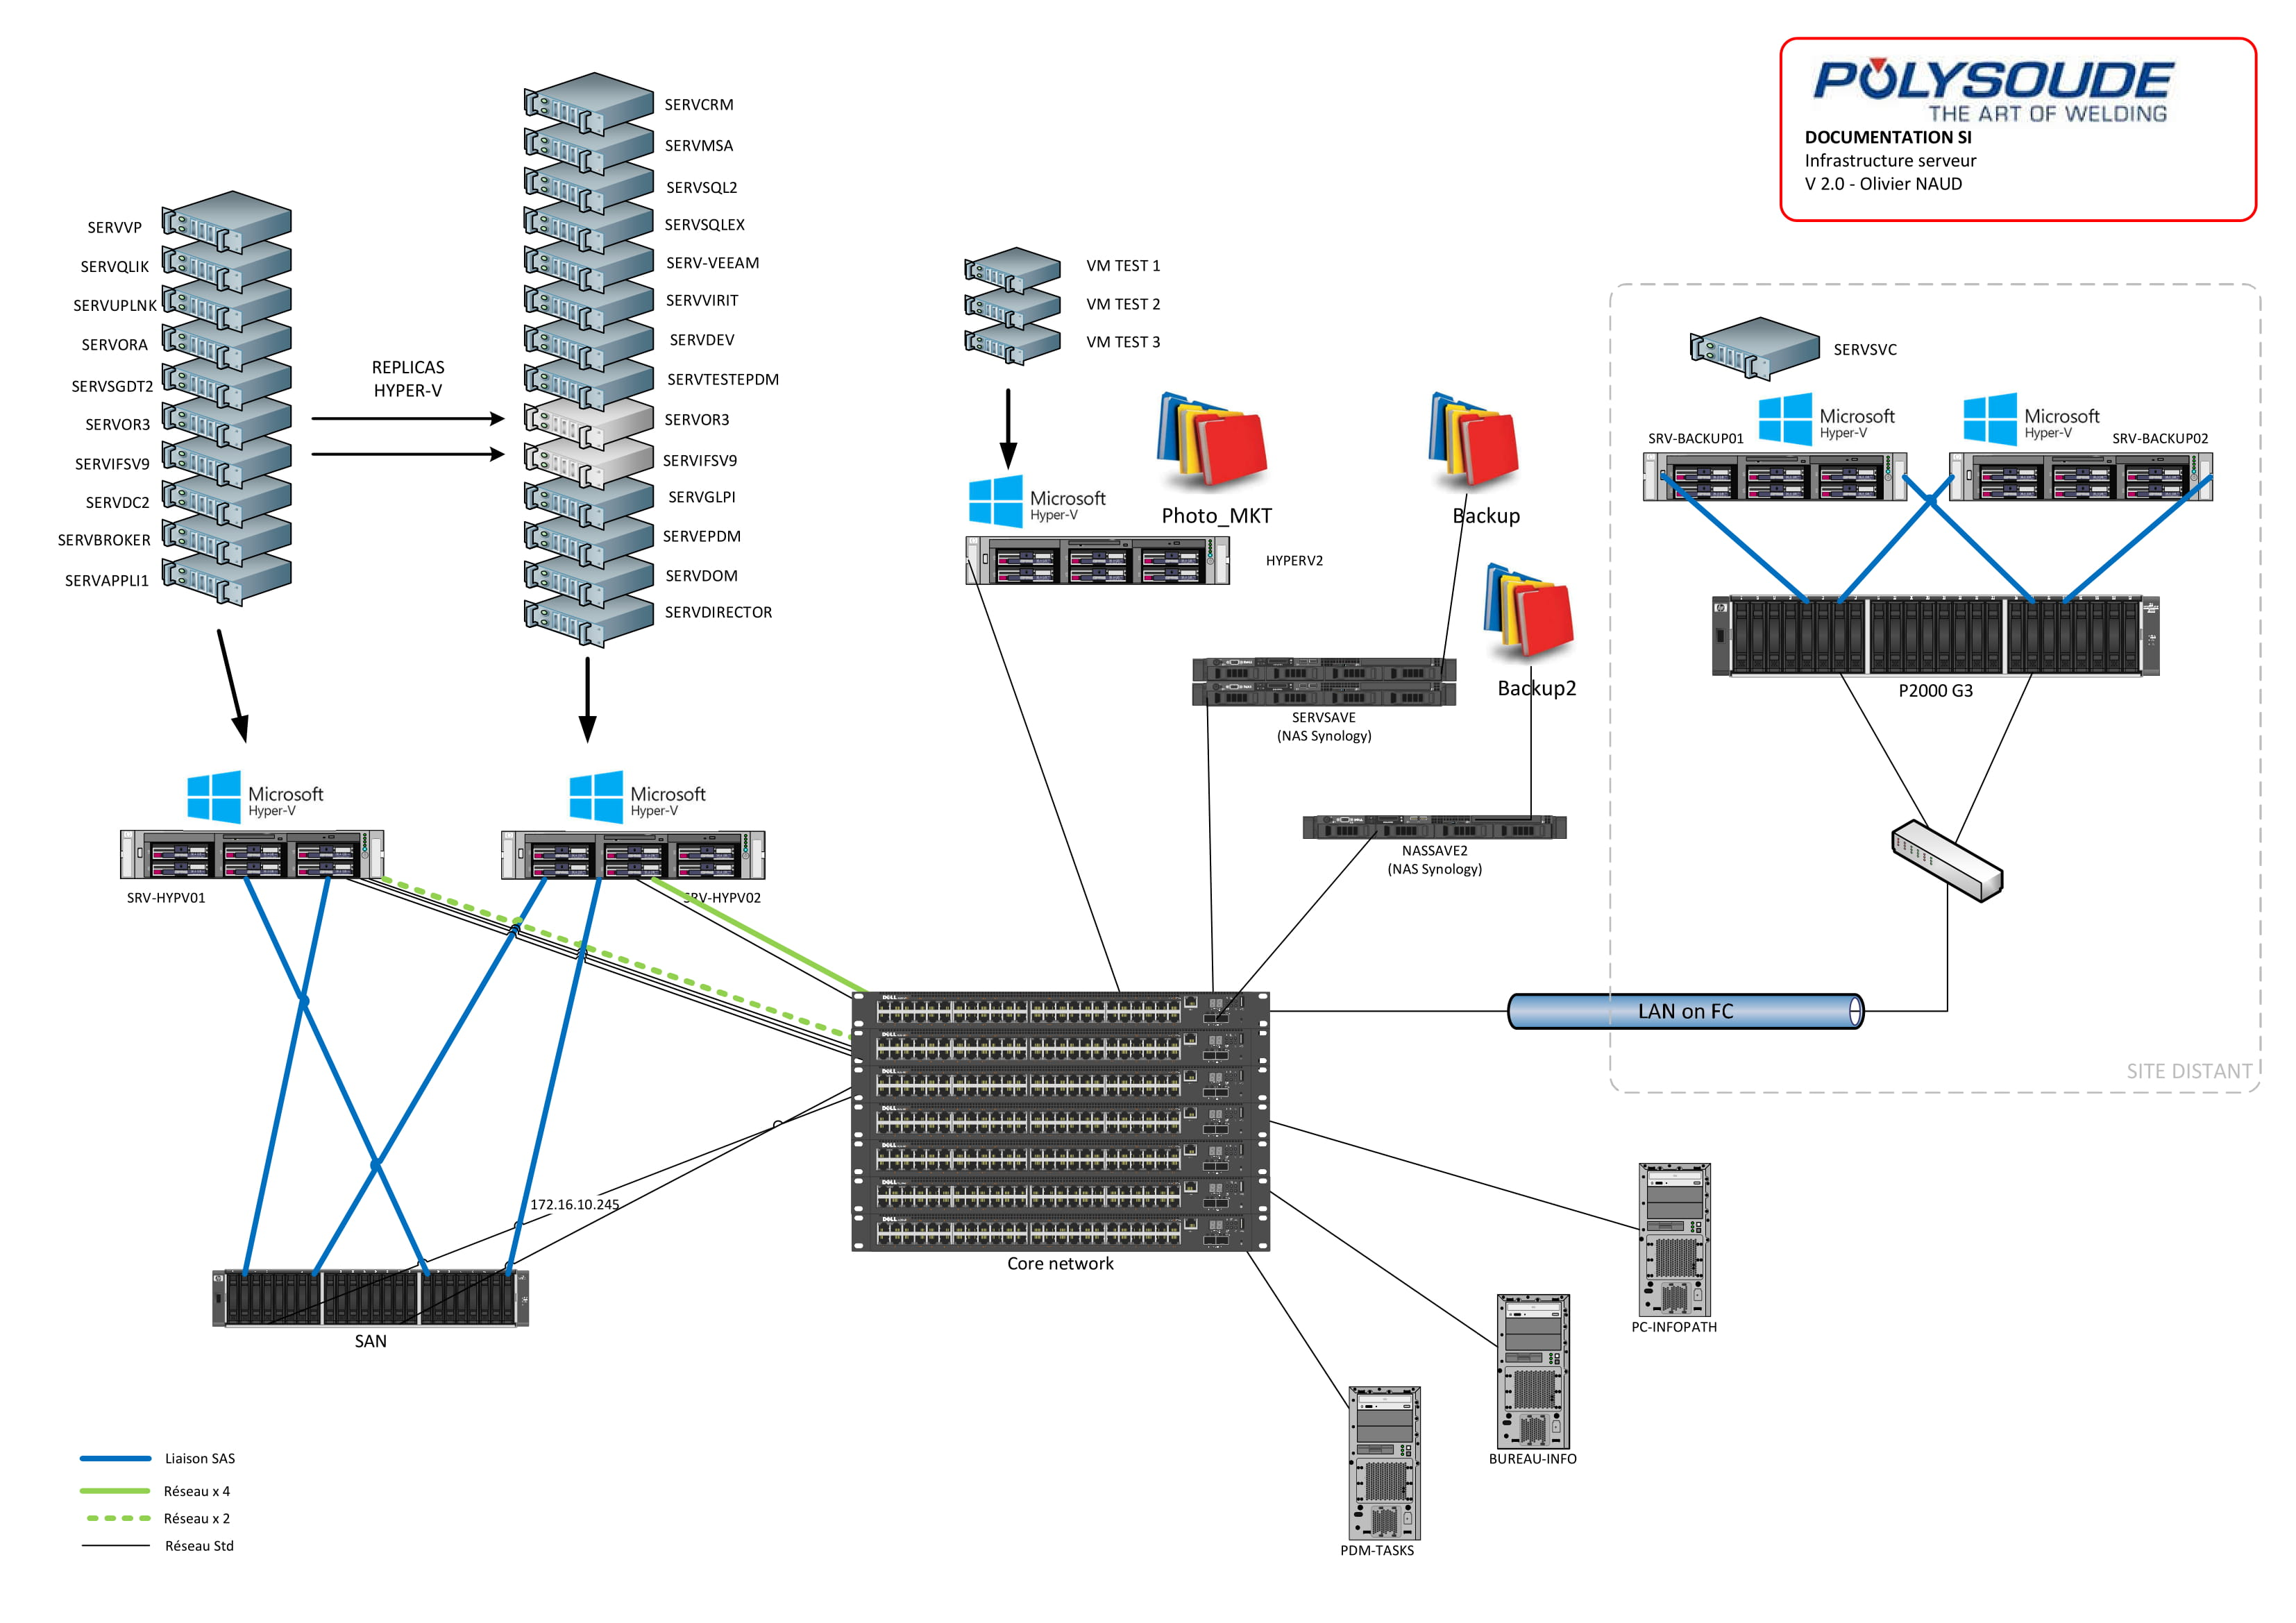
\includegraphics[scale=0.2]{Ressources/Reseau.jpg}}
\newpage

% Type matériel réel / Virtuel
\subsubsection{Postes Fixes}
% ### 1 ###
\begin{wrapfigure}{c}{7cm}
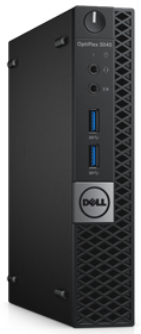
\includegraphics[scale=0.4]{Ressources/Materiel/3040.png}\vspace{-2cm}
\end{wrapfigure}
\paragraph{}\textbf{Dell OptiPlex 3040 Micro :} \\
\begin{itemize}
\item \textbf{CPU :} Intel Core i3
\item \textbf{RAM :} 8 Go
\item \textbf{OS :} Windows 7 / Windows 10
\item \textbf{Disque Dur :} 256 Go SDD / 500 Go HDD
\item \textbf{Quantité :} 41 unités
\\ \\ \\ \\
\end{itemize}
%%%%%%%%%%%%%%%
\begin{wrapfigure}{c}{7cm}
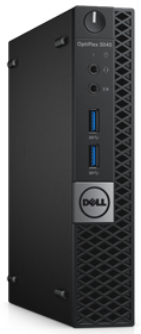
\includegraphics[scale=0.4]{Ressources/Materiel/3040.png}\vspace{-2cm}
\end{wrapfigure}
\paragraph{}\textbf{Dell Optiplex 3050 Micro :} \\
\begin{itemize}
\item \textbf{CPU :} Intel Core i5-7500T // Intel Core i3-7100T
\item \textbf{RAM :} 8 Go
\item \textbf{OS :} Windows 7 / Windows 10
\item \textbf{Disque Dur :} 256 Go SSD // 500 Go HDD
\item \textbf{Quantité :} 2 unités
\\ \\ \\ \\
\end{itemize}
%%%%%%%%%%%%%%%
\begin{wrapfigure}{c}{7cm}
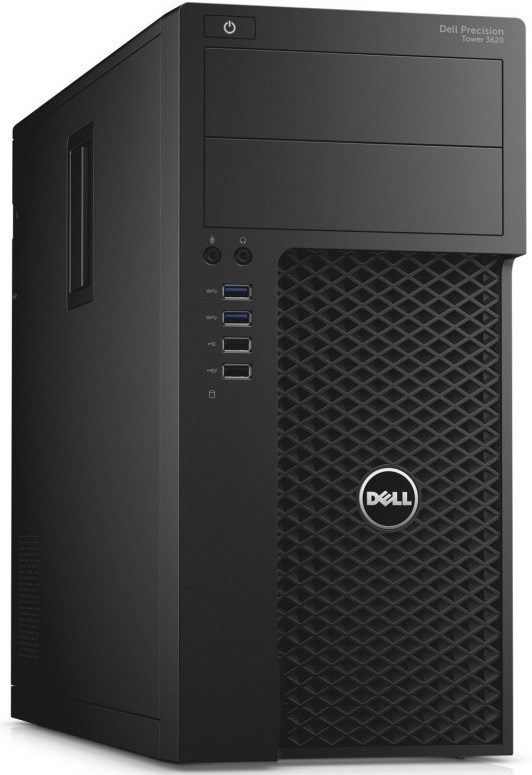
\includegraphics[scale=0.3]{Ressources/Materiel/3620.jpg}\vspace{-2cm}
\end{wrapfigure}
\paragraph{}\textbf{Dell Precision 3620 :} \\
\begin{itemize}
\item \textbf{CPU :} Intel Core i7-6700
\item \textbf{RAM :} 8 Go
\item \textbf{OS :} Windows 7
\item \textbf{Disque Dur :} 256 Go SSD // 500 Go SSHD
\item \textbf{Quantité :} 12 unités
\\ \\ \\ \\
\end{itemize}
\newpage

\subsubsection{Postes Portables}
% ### 2 ###
\begin{wrapfigure}{c}{7cm}
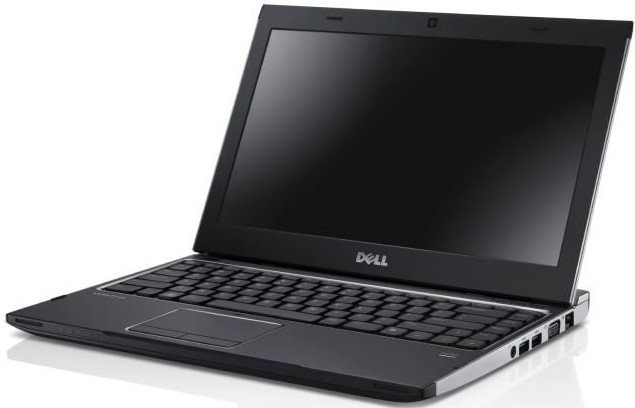
\includegraphics[scale=0.4]{Ressources/Materiel/V131.jpg}\vspace{-2cm}
\end{wrapfigure}
\paragraph{}\textbf{Dell Vostro V131 :} \\
\begin{itemize}
\item \textbf{CPU :} Intel Core i5-2450M
\item \textbf{RAM :} 8 Go
\item \textbf{OS :} Windows 7
\item \textbf{Disque Dur :} 500 Go HDD
\item \textbf{Quantité :} 13 unités
\\ \\ \\ \\
\end{itemize}
%%%%%%%%%%%%%%%
\begin{wrapfigure}{c}{7cm}
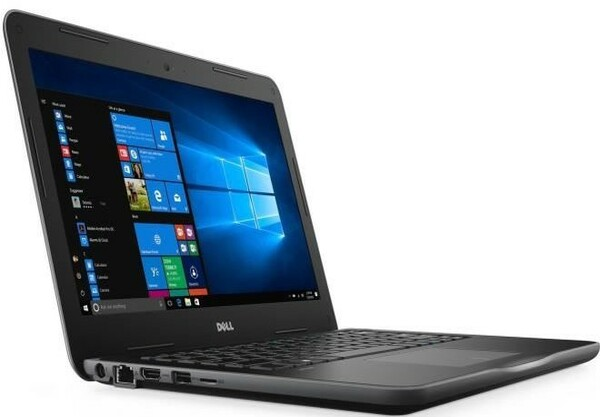
\includegraphics[scale=0.4]{Ressources/Materiel/L3380.jpg}\vspace{-2cm}
\end{wrapfigure}
\paragraph{}\textbf{Dell Latitude 3380 :} \\
\begin{itemize}
\item \textbf{CPU :} Intel Core i5-7200U
\item \textbf{RAM :} 8 Go
\item \textbf{OS :} Windows 7
\item \textbf{Disque Dur :} 256 Go SSD / 500 Go HDD
\item \textbf{Quantité :} 17 unités
\\ \\ \\ \\
\end{itemize}
%%%%%%%%%%%%%%%
\begin{wrapfigure}{c}{7cm}
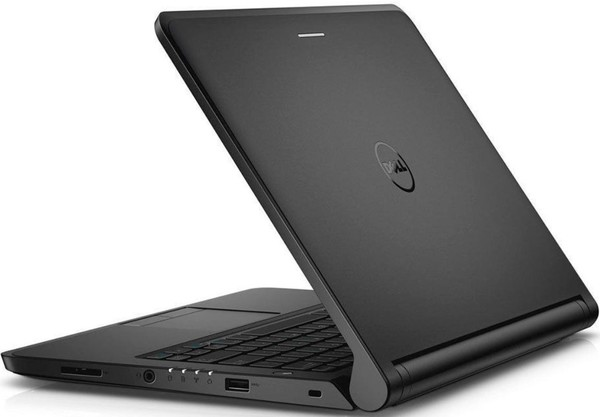
\includegraphics[scale=0.4]{Ressources/Materiel/L3350.jpg}\vspace{-2cm}
\end{wrapfigure}
\paragraph{}\textbf{Dell Latitude 3350 :} \\
\begin{itemize}
\item \textbf{CPU :} Intel Core i5-4210U
\item \textbf{RAM :} 8 Go
\item \textbf{OS :} Windows 10
\item \textbf{Disque Dur :} 256 Go SSD
\item \textbf{Quantité :} 14 unités
\\ \\ \\ \\
\end{itemize}
%%%%%%%%%%%%%%%
\begin{wrapfigure}{c}{7cm}
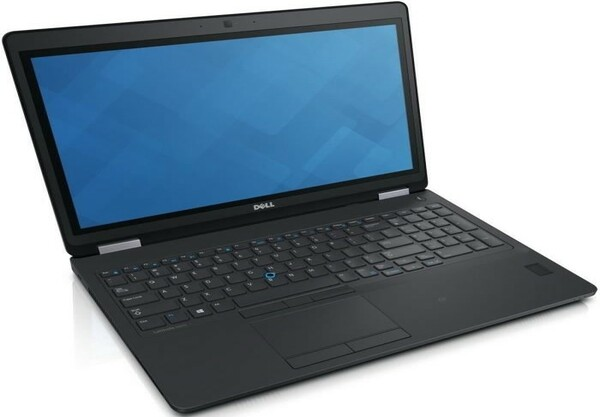
\includegraphics[scale=0.4]{Ressources/Materiel/LE5570.jpg}\vspace{-2cm}
\end{wrapfigure}
\paragraph{}\textbf{Dell Latitude E5570 :} \\
\begin{itemize}
\item \textbf{CPU :} Intel Core i7-6820HQ
\item \textbf{RAM :} 8 Go
\item \textbf{OS :} Windows 10
\item \textbf{Disque Dur :} 256 Go SSD
\item \textbf{Quantité :} 4 unités
\\ \\ \\ \\
\end{itemize}
%%%%%%%%%%%%%%%
\begin{wrapfigure}{c}{7cm}
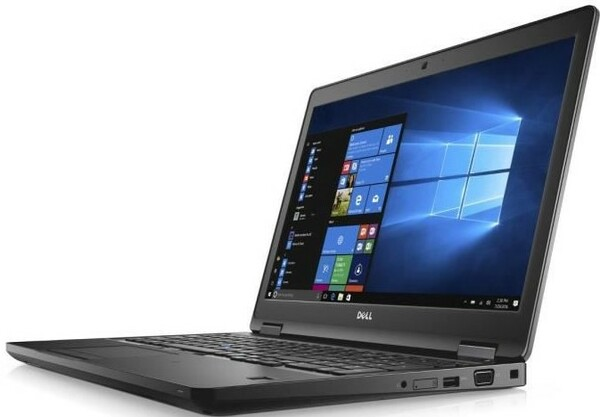
\includegraphics[scale=0.4]{Ressources/Materiel/L5580.jpg}\vspace{-2cm}
\end{wrapfigure}
\paragraph{}\textbf{Dell Latitude 5580 :} \\
\begin{itemize}
\item \textbf{CPU :} Intel Core i7-6820HQ
\item \textbf{RAM :} 8 Go
\item \textbf{OS :} Windows 10
\item \textbf{Disque Dur :} 256 Go SSD
\item \textbf{Quantité :} 5 unités
\\ \\ \\ \\ \\
\end{itemize}
%%%%%%%%%%%%%%%
\begin{wrapfigure}{c}{7cm}
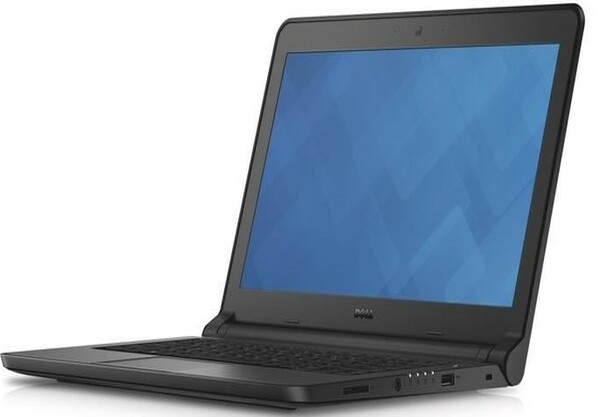
\includegraphics[scale=0.4]{Ressources/Materiel/L3340.jpg}\vspace{-2cm}
\end{wrapfigure}
\paragraph{}\textbf{Dell Latitude 3340 :} \\
\begin{itemize}
\item \textbf{CPU :} Intel Core i5-4210U
\item \textbf{RAM :} 8 Go
\item \textbf{OS :} Windows 10
\item \textbf{Disque Dur :} 256 Go SSD
\item \textbf{Quantité :} 23 unités
\\ \\ \\ \\
\end{itemize}
%%%%%%%%%%%%%%%
\begin{wrapfigure}{c}{7cm}
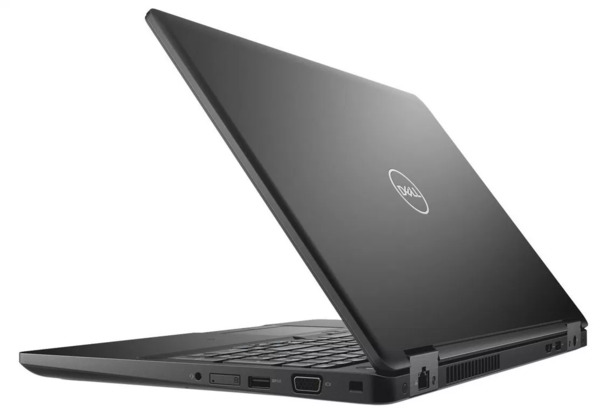
\includegraphics[scale=0.35]{Ressources/Materiel/L5591.jpg}\vspace{-2cm}
\end{wrapfigure}
\paragraph{}\textbf{Dell Latitude 5591 :} \\
\begin{itemize}
\item \textbf{CPU :} Intel Core i5-4210U
\item \textbf{RAM :} 8 Go
\item \textbf{OS :} Windows 10
\item \textbf{Disque Dur :} 256 Go SSD
\item \textbf{Quantité :} 14 unités
\\ \\ \\ \\
\end{itemize}
%%%%%%%%%%%%%%%
\begin{wrapfigure}{c}{7cm}
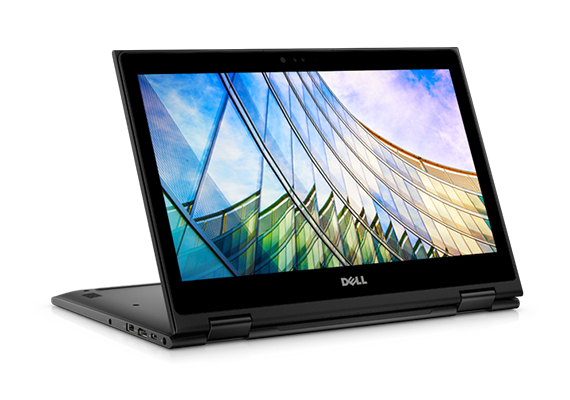
\includegraphics[scale=0.35]{Ressources/Materiel/3390.png}\vspace{-2cm}
\end{wrapfigure}
\paragraph{}\textbf{Dell Latitude 3390 2-in-1 :} \\
\begin{itemize}
\item \textbf{CPU :} Intel Core i5-8250U
\item \textbf{RAM :} 16 Go
\item \textbf{OS :} Windows 10
\item \textbf{Disque Dur :} 256 Go SSD
\item \textbf{Quantité :} 4 unités
\\ \\ \\ \\
\end{itemize}

% ##### Page 6 #####
\newpage
\section{Objectif(s) du stage}

Lors du 1\ier{} passé chez POLYSOUDE, le responsable informatique voulait une personne autonome, vif et capable d'agir en restant calme (en fonction de la demande) et travailler en équipe.
\\ \\
Pour moi, c'était la 1\ier fois que j'avais ce genre de mission et de responsabilité au sein d'un parc de plus de 150 postes et surtout avec une équipe.
\\ \\
Les tâches qui m'ont été confiées au fil du temps étaient : 
\begin{itemize}
    \item Répondre aux appels téléphonique pour une intervention par téléphone.
    \item Assurer la gestion de parc.
    \item Former les utilisateurs sur les outils / matériels mis à disposition.
    \item Utiliser l'outil de ticketing GLPI.
    \item Réinitialiser les mots de passe des utilisateurs.
    \item Déploiement de poste.
    \item Gestion des demandes matérielles.
    \item Ouvrir des tickets de support chez nos différents prestataires.
\end{itemize}

% ##### Page 7 ######
\newpage
\section{Environnement du stage}
Les postes des utilisateurs étaient souvent dans leurs bureaux ou sur leurs lieux de travail dans l'atelier. \\

% ##### Page 8 ######
\newpage
\section{Présentation des principales activités \\ \& réalisation durant le stage}
\subsection{Support utilisateur}

\begin{figure}[!h]
\centering
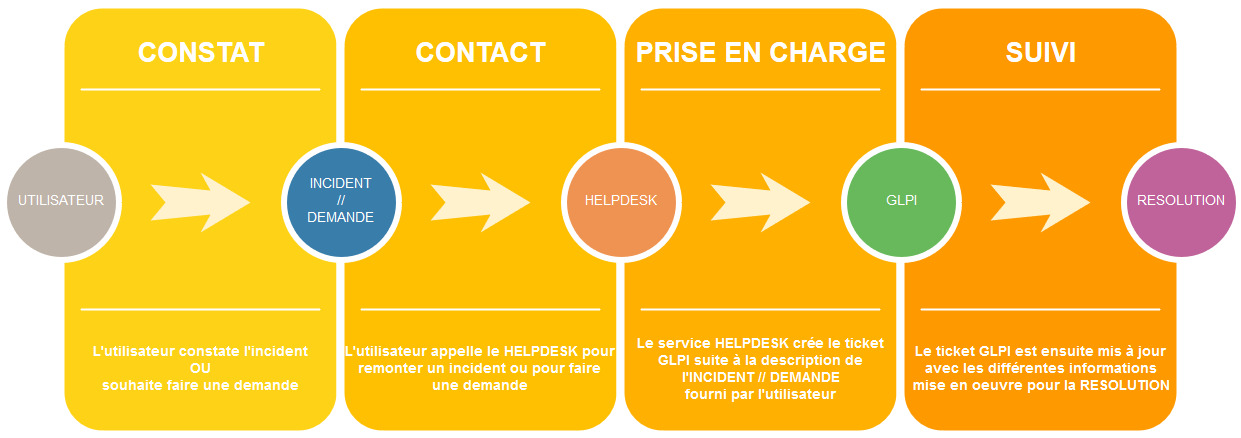
\includegraphics[scale=0.42]{Ressources/GLPI.jpg}
\caption{Schéma de support}
\end{figure}

Dès le besoin d'assistance, les utilisateurs appelant le numéro du \textbf{Heldesk}. Ce numéro est utilisé par un groupe d'appel géré par \textbf{Shoreware Director}\footnote{Serveur VOIP} pour faire une boucle sur le téléphone de mon collègue ainsi que le mien (DECT ou IPPHONE). \\

En détail du schéma ci-dessus, voici un exemple de notre démarche de support :

\begin{enumerate}
\item \textbf{L'utilisateur} constate qu'il n'arrive pas à ouvrir sa session Windows.
\item Cet utilisateur va appelé le \textbf{Heldesk} pour avoir l'un des 2 techniciens support et ainsi prend en charge l'incident.
\item \textbf{L'un des techniciens support} prend en charge l'appel en posant les bonnes questions (ouvertes ou fermées).
\item Le technicien qui à prit l'appel va ouvrir un ticket sous \textbf{GLPI} en mettant le plus de détails sur l'incident.
\item  Si c'est possible, le technicien va \textbf{intervenir} à distance ou sinon sur site jusqu'à la \textbf{résolution} de l'incident en décrivant toutes les étapes sous le ticket ouvert précedemment.
\end{enumerate}

\newpage

% ##### Page 9 ######
\subsection{Déploiement de poste}
\subsubsection{L'idée de base}

Dans le cadre d’une nouvelle installation de Windows 7 ou de Windows 10, nous utilisons un moyen de déploiement nommé \textbf{MDT}  \footnote{Microsoft Deployment Toolkit} et grâce à cet outil, il est facile de créer son image et déployer Windows sur les nouveaux postes.

Cela permet d’automatiser le(s) installation(s) système ainsi que les logiciels sur un ou plusieurs postes à la fois.
\subsubsection{Préparation post-déploiement}
\begin{enumerate}
    \item \textbf{Les pré-requis :}
\end{enumerate}
•	Un support d’installation (Clé USB, Disque dur externe) bootable. \\
•	Une connexion filaire. \\
•	Un ordinateur à déployer (PC Portable ou Fixe). \\
•	La roadmap

\begin{enumerate}
\setcounter{enumi}{1}
    \item \textbf{La roadmap :}
\end{enumerate}

•	Les informations de l’utilisateur ainsi que le nom du poste. \\
•	Quel type de système d’exploitation à installer.\\
•	Les diverses étapes de configuration à faire.\\
•	Les logiciels à installer (avec le master et manuellement).\\
•	La configuration du profil utilisateur.\\
•	Et si besoin, une récupération de données à faire (si c’était un poste à refaire).

\subsubsection{Processus de déploiement}
En ayant validé toutes les informations « post-déploiement », cela va commercer les différents processus de déploiement en commençant par : \\
\begin{enumerate}
    \item Le formatage et le partitionnement du disque prédéfini dans la console MDT : Dans notre cas, c’est le disque 0 en table GPT.
    \item L’injection des pilotes : En fonction de la marque et du modèle de l’ordinateur, les pilotes seront copiés et installés.
    \item Installation du système d’exploitation : l’OS est prédéfini depuis la console MDT en utilisant une image « .WIM » fourni avec le CD d’installation ou une image ISO d’installation.
    \item Installation des bundles d’applications : Les applications voulues pour qu’elles soient automatiquement installées.
    \item Scripts de configuration pour divers paramétrages d’utilisation.
    \item Quelques redémarrages …
    \item … Et une fenêtre montrant si le déploiement s’est bien passé ou s’il y a eu des erreurs.
\end{enumerate}	

\newpage

\section{Conclusion}
Ces différentes expériences m’ont permis d’apprendre, d’approfondir et d’intégrer mon goût pour cet univers technologique au sein d’un environnement professionnel. Cela m’a également permis de développer les qualités d’écoute et de communication grâce aux contacts relationnelles avec les utilisateurs. \\

L’objectif principal de cette démarche est d’élargir les compétences techniques dans le domaine du support informatique. Les périodes en entreprise m’ont appris des méthodes d’organisation. J’ai aussi gagné en autonomie et surtout sur la confiance en soi en étant fière des missions réalisées en entreprise ! \\

C’est pour cela que je considère la formation de \textbf{Technicien Supérieur de Support en Informatique} au sein de l’ENI comme un choix important pour perfectionner mes méthodologies, mes compétences ainsi que mon sens des responsabilités. \\
\end{document}